%%This is a test of the 'beamer' class for LaTeX

\documentclass[pdf]{beamer}

\mode<presentation>{\usetheme{Warsaw}}
\usecolortheme{seahorse}
\usepackage{graphicx}
\graphicspath{ {.} }

%%preamble

\title{Verifying the Accuracy of sleep() and usleep()}
\author{Kevin Bloom}


\begin{document}

%%title frame

\begin{frame}

  \titlepage

\end{frame}

%%normal frame

\begin{frame}{Objectives}


  Using the ZYBO Private Timer \& DSO:
  \pause
  \begin{itemize}

  \item Verify the accuracy of both functions

    \pause

  \item Compare accuracy of the private timer and DSO

    \pause

  \item Determine delay to set a pin high/low

  \end{itemize}
  

\end{frame}

\begin{frame}{Functional Block Diagram}

  \centering
  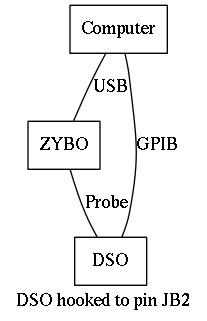
\includegraphics[width=50mm]{block-diagram.png}

\end{frame}

\begin{frame}{Functionality}

  \begin{itemize}
  \item User inputs value in C\#
  \item C\# sends value to the ZYBO
  \end{itemize}
  
  \pause

  \begin{itemize}
  \item ZYBO uses this value as the sleep time
  \item ZYBO starts private timer, sets JB2 high, and sleeps
  \item DSO collects its data
  \end{itemize}
  
  \pause
  
  \begin{itemize}
  \item Once finished, the ZYBO sends sleep value to C\#
  \item C\# reads all data off the DSO
  \item C\# finds all data that is high
  \end{itemize}

\end{frame}

\begin{frame}{Tests}

  20 Total Tests
  \begin{itemize}
  \item 10 tests per function
  \item Values per test range from low to high
  \item 10 data points per test
  \end{itemize}
    
\end{frame}

\end{document}

